\section*{\koroibot\ Key Performance Indicator (KPI)}
\label{sec:keyperf}

\begin{figure}[ht]
\centering
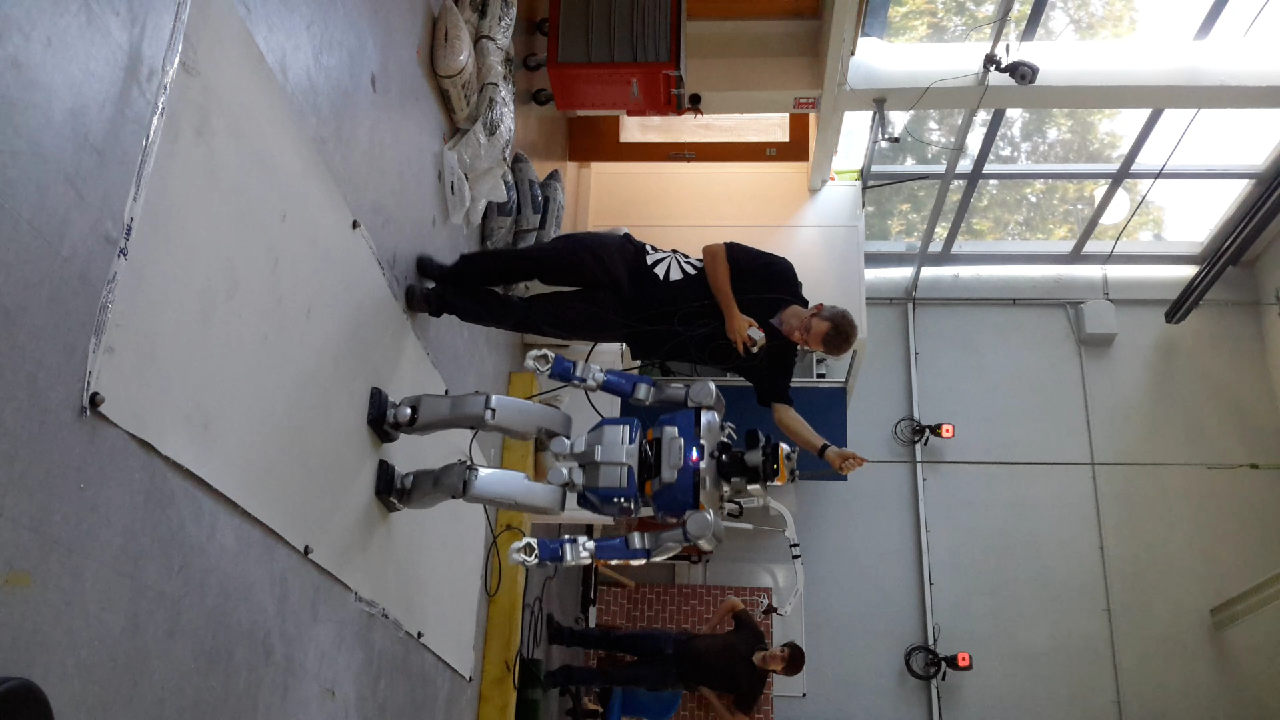
\includegraphics[angle=90, height=0.2\linewidth]{figures/ground.png}
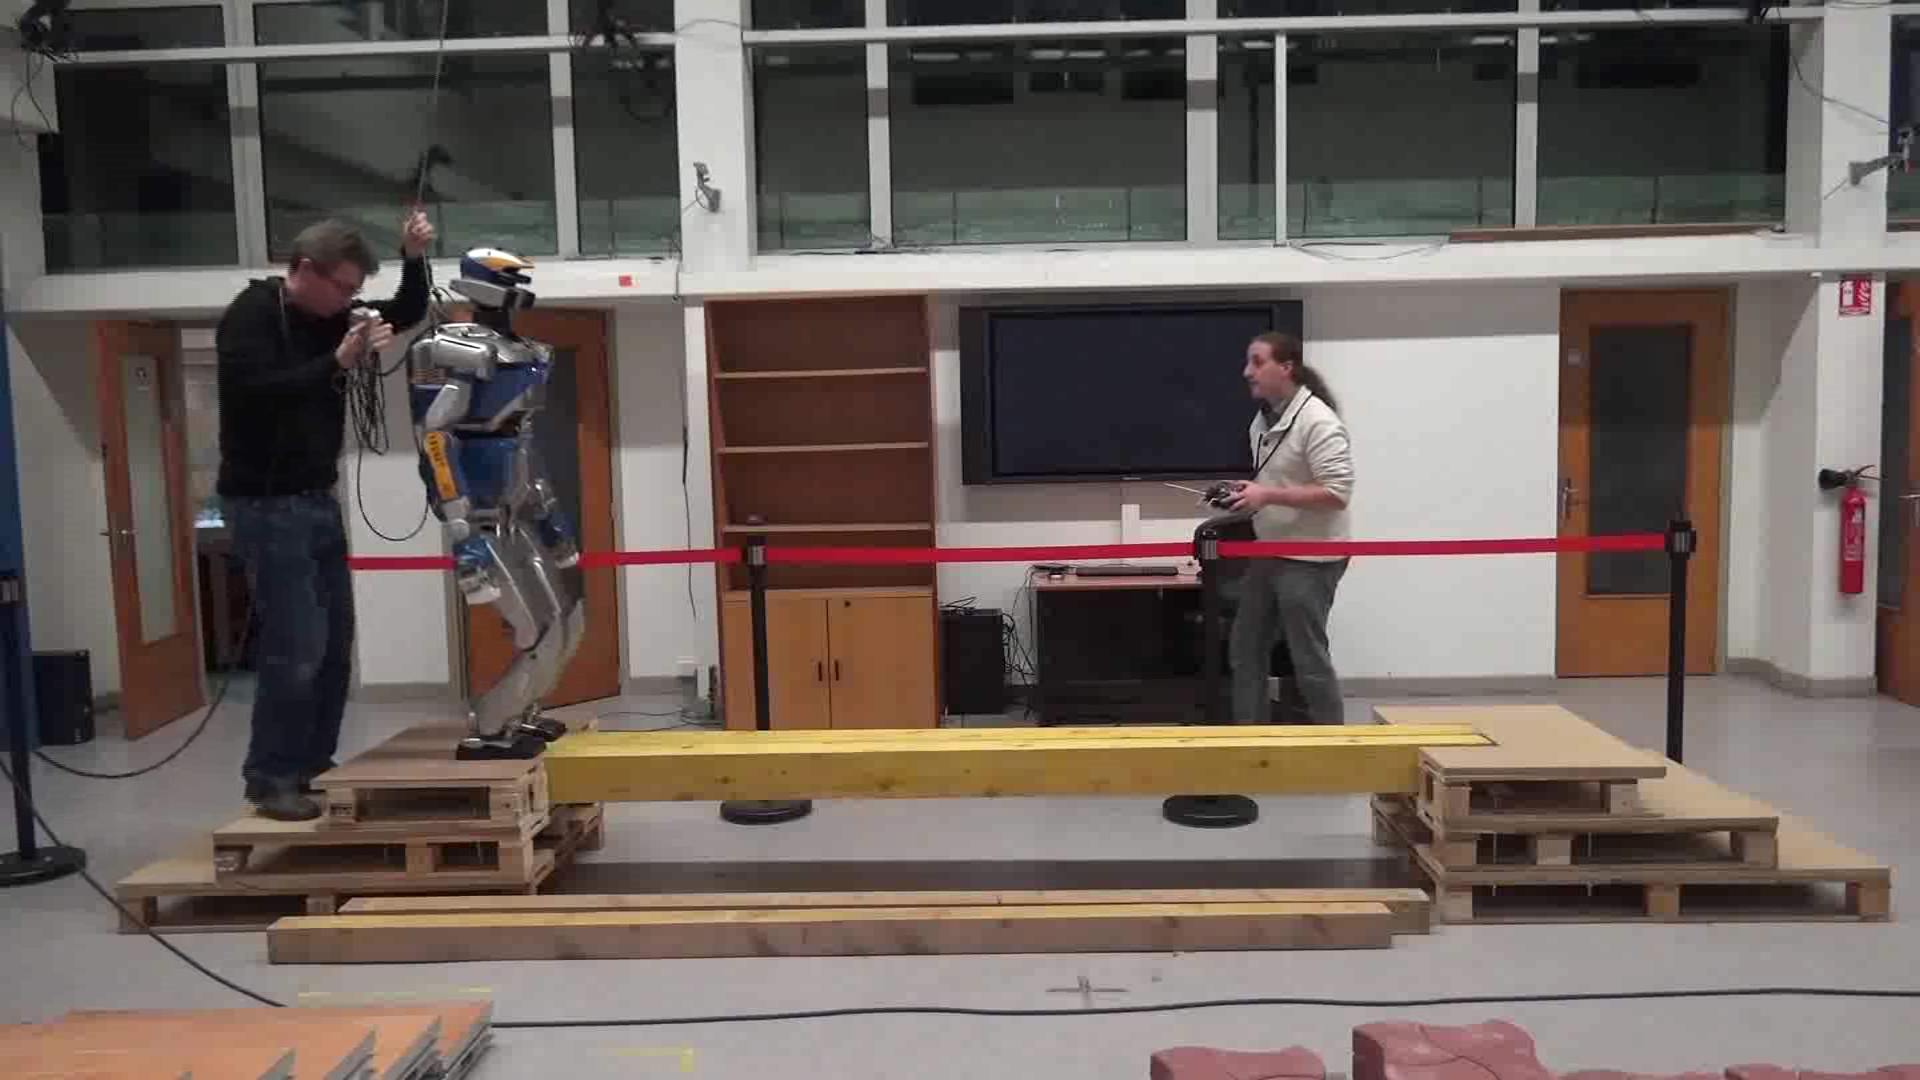
\includegraphics[height=0.2\linewidth]{figures/beam.png}\\[1ex]
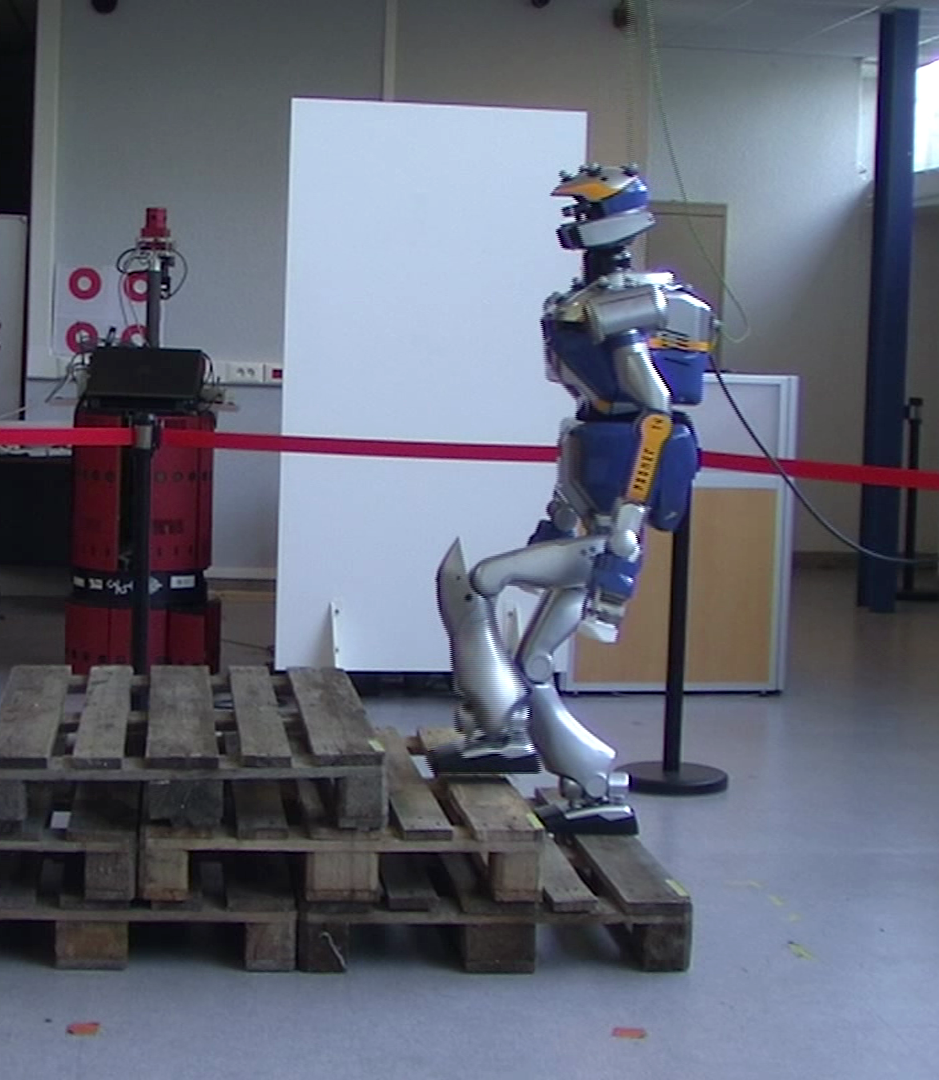
\includegraphics[height=0.2\linewidth]{figures/upstair.png}
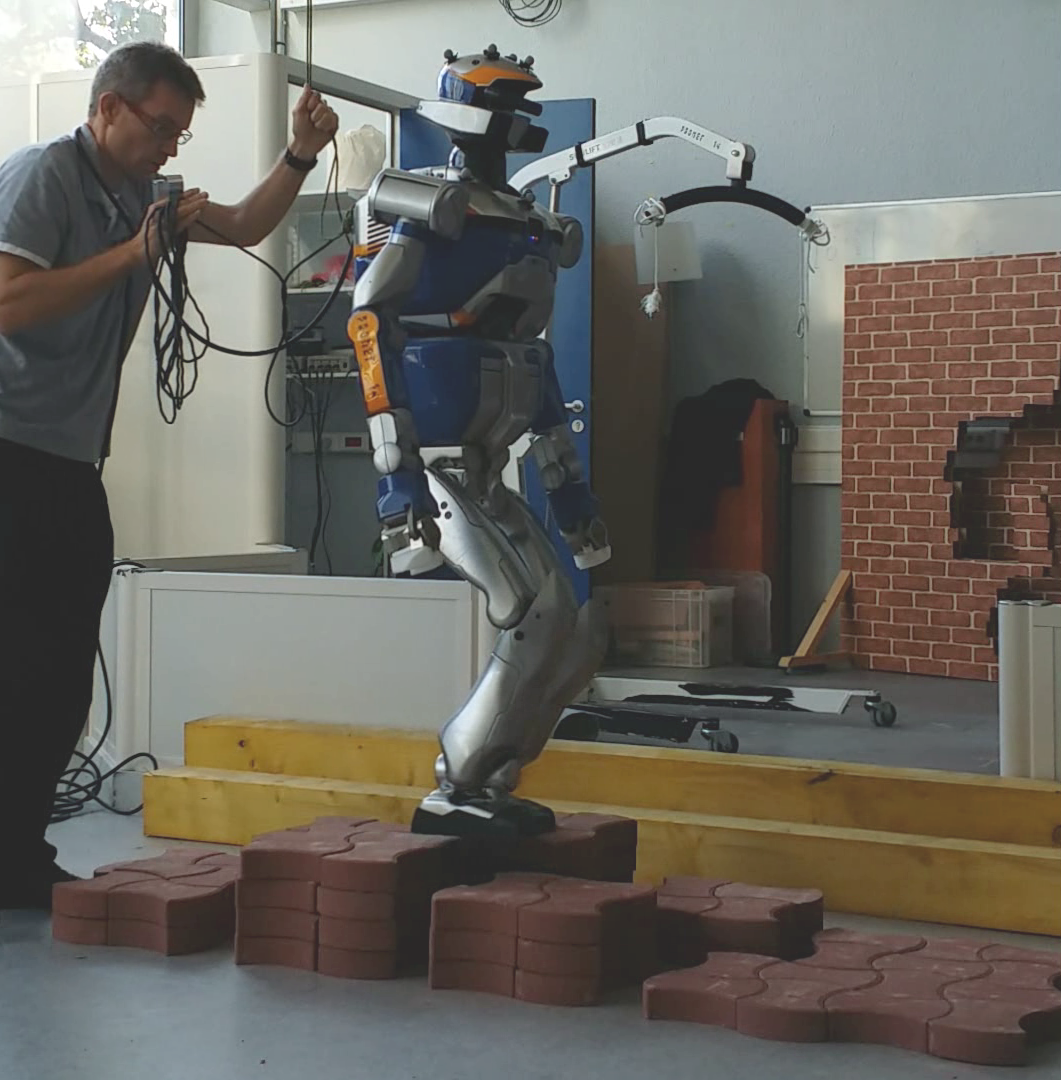
\includegraphics[height=0.2\linewidth]{figures/steppingstones.png}
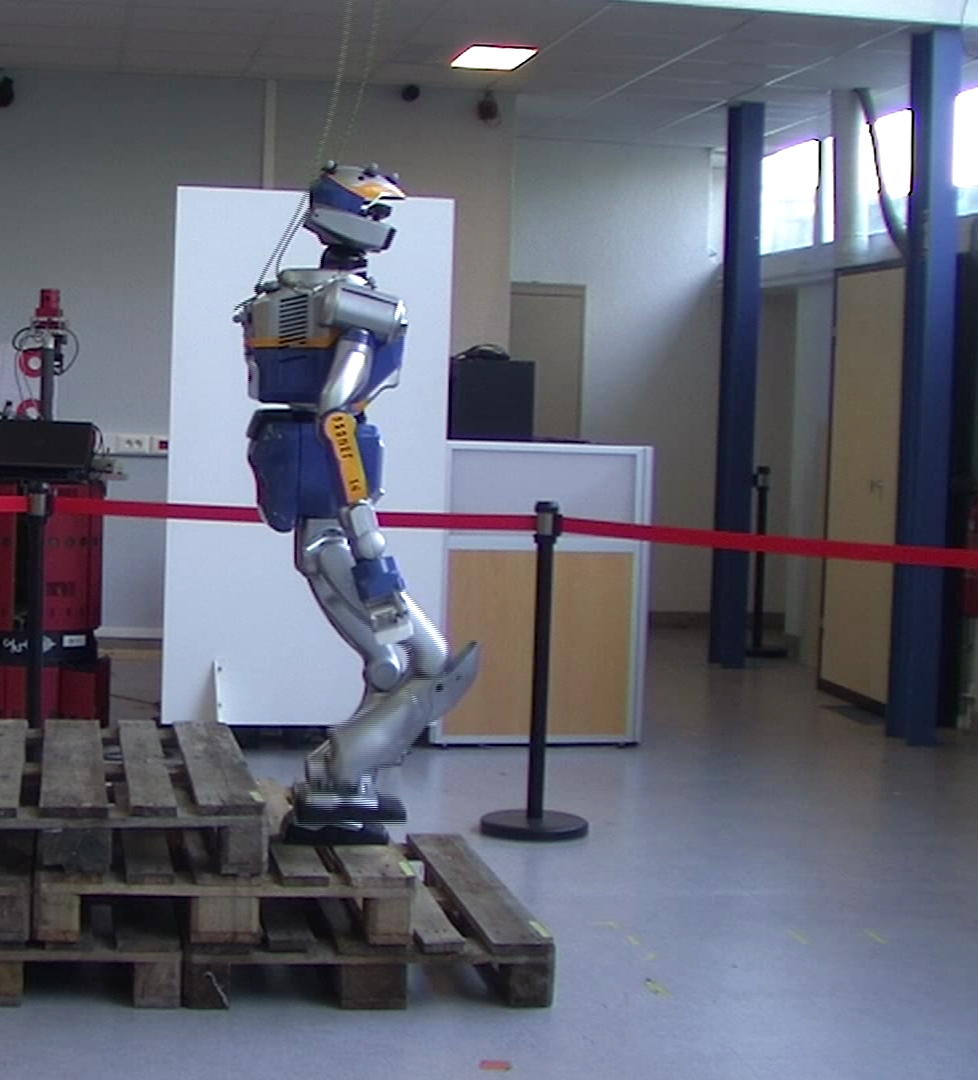
\includegraphics[height=0.2\linewidth]{figures/downstair.png}
\caption{Sample of the experimental setup of the \koroibot\ project in LAAS-CNRS}
\label{fig:koroibot:setupreal}
\end{figure}


In the \koroibot\ project we used key performance indicators (KPI) to analyze the behavior of the robot at the beginning and at the end of the project.
These results lead us toward the improvements to be made.
In 2013 the algorithm mostly used and implemented on HRP-2 in LAAS-CNRS where the walking pattern generators described in \cite{Morisawa:ICRA:2007} and in \cite{herdt:iros:2010}.
The performance indicators chosen were:
\begin{list}{ \arabic{point}.}{%
		\usecounter{point}%
		\setlength{\topsep}{5pt}%
		\setlength{\itemsep}{0pt}%
		\setlength{\parsep}{0pt}%
		\setlength{\labelwidth}{3.em}%
		\setlength{\leftmargin}{2em}%
		\setlength{\labelsep}{0.5em}%
	}

\item[\bluesquare] the execution time $T_M$,
\item[\bluesquare] the time to compute the motion $T_{think}$,
\item[\bluesquare] the total energy consumed during a walking distance $D$,
\begin{equation*}
E_{walk} = \int_{t_b{begin}}^{t_{end}} \tau \omega dt + \int_{t_b{begin}}^{t_{end}} R k_c^2
\tau^2 dt \;,\;\;\; \tilde{E}_{walk} = E_{walk}/D 
\end{equation*}
with $E_{walk}$ being the total energy consumed counting the integral over time of the mechanical power and the electrical power dissipated by the motors. $\tau$ and $\omega$ being respectively the joint torques and velocities, and $R$ with $k_c$ being respectively the motor resistances and torque constants.
\item[\bluesquare] the mechanical energy consumed during a walking distance $D$,
\begin{equation*}
E_{meca} = \int_{t_{begin}}^{t_{end}} \tau \omega dt
 \;,\;\;\; \tilde{E}_{meca} = E_{meca}/D 
\end{equation*}
with $E_{meca}$ being the integral over time of the mechanical power,
\item[\bluesquare] the deviation from the planned trajectory $P_{T_r}$,
\item[\bluesquare] and the maximum speed reached $V_{max}$.
\end{list}
The trajectories were generated offline and repeatedly played on the robot to analyze their robustness.
Samples of the experimental setups can be seen in Fig.~\ref{fig:koroibot:setupreal}.

\subsection*{Straight walking}

\begin{tabular}{|c|c|c|c|c|c|c|c|}
\hline
   $T_M$ & $T_{think}$ & $\tilde{E}_{walk}$ & $\tilde{E}_{meca}$ &
   $P_{T_r}^\theta$ & $P_{T_r}^x$ & $P_{T_r}^y$ & $V_{max}$\\
\hline
   $7\,s$ & $2\,s$ & $47250\,J/m$ & $47070\,J/m$ &
   $-0.0013\,rad$ & $0.026\,m$ & $0.052\,m$ & $0.125\,m/s$\\
\hline
\end{tabular}
\\

From these results we can observe that the HRP-2 is very repeatable.
However the room for improvement lies in the maximum velocity speed which is quiet slow.

\subsection*{3D walking}

Here 3D walking means walking on flat ground but possibly a different height, like stair case or stepping stones.
The walking pattern generators \cite{Morisawa:ICRA:2007,herdt:iros:2010} normally does not allow the possibility to perform movement such as climbing stairs.
For this reason we designed smooth feet 3D trajectories using B-Splines and a prior knowledge of the environment.
Empirically we found trajectories that fits kinematics and dynamics constraints.
The results of these implementation is shown in \cite{naveau:ichr:2014}

\subsection*{Walking in stairs or on stepping stones}

\begin{tabular}{|c|c|c|c|c|c|}
\hline
   $T_M$ & $T_{think}$ & $\tilde{E}_{walk}$ & $\tilde{E}_{meca}$ &
   $P_{T_r}$ & $V_{max}$ \\
\hline
   $7\,s$ & $2\,s$ & $256150,J/m$ & $255270\,J/m$ &
   - & - \\
\hline
\end{tabular}
\\

This results shows the KPI value when the robot goes up the stair case.
The important consumption of energy during the climbing up stairs is to be noted.
Diminishing this power consumption is an important factor as it will decrease the loss of electrical energy and the mechanical stress on the robot.
The repeatability of this experiment is around $40\,\%$.

The results of the KPI, when the robot goes downstairs, are very similar to the going up experiment.
The repeatability of the going down stairs motion is around $95\,\%$.
The only point is that the global energy is twice lower than when the robot is going up.
The reason is that it is less fighting the gravity while going down.

For the stepping stone experiment the KPI were also very similar to the above two experiments.
Though, as expected, the energy consumption is between going up and going down stairs.
The repeatability of this experiment is around $50\,\%$.

\subsection*{Walking on a beam}

The major problem of this experiment is its success rate which is around $20\,\%$.
In order to improve this rate we need to take care of the robot balance and the robot feet placement.
Indeed the two main reasons of the robot fall were the default of balance on the beam and the drift which is important as the beam length is $3\,m$ long.

\subsection*{Step over obstacles}

This manipulation has not been performed in the frame of this thesis.
It is a work published in \cite{koch:ichr:2014} already presented in the above sections.
The improvement to be made here is on the computation time.
As explained before in subsection {"Whole body formulations"}, these trajectory took several hours to be computed.
